\chapter{Evaluation}
\label{ch:Evaluation}

\section{Research}

% TODO cite arxiv and google scholar so it is listed in references
Searching information always is a key element in research. Therefor, \href{arxiv.org}{arXiv} and \href{scholar.google.de}{Google Scholar} were used in order to find suitable reading.\\
It proofed to be difficult to find such papers using keywords such as "grid-based" or "geographic", because most of the results referred to either other grids, such as in Smart Grid, or completely different geographic research subjects.\\
As weather data from the \acrshort{ecmwf} is used in this thesis, which is grid based, one solution was to search for "ECMWF", as this type of data is widely used within the research field of energy.\\

also used \href{base-search.net}{BASE} which proposed "energy network geographic data" after searching a bit, I came to the term "energy network ecmwf" which gave some hits.\\
One criteria is the title which tells much about the subject of the work. If the title implies both, working with geographic or grid-based data and also has a connection to the field of energy networks, it might be suitable for this work.\\
Another one is the abstract and/or introduction which tells some more details about the paper. If there are some points about applying geographic data in algorithms to forecast some power production or demand, it is most likely that this paper contains some valuable information for this thesis.\\

\section{Data}

\subsection{ECMWF}

The data used in this thesis originates from \acrshort{ecmwf}, which is a research institute that produces global numerical weather predictions and other data.\\
It is time series based and for each timestamp there is a 2-dimensional array referred to by longitude and latitude respectively.\\

It must be mentioned that, as the data used has been reanalized, the expected error is likely to be smaller than if working with real-time data.\\

As data parameters there are also longitude and latitude, where the longitude is chosen to be from 5.5 to 15.5 and the latitude from 47 to 55.5. As the resolution of the used grid is at 0.25°, this results in a total of 1435 grid points per timestamp. As the range of the data from \acrshort{ecmwf} extends from 2015/1/1 to 2019/3/31(TODO update), there is a total of 1551 days with each 12 timestamps due to the 2 hours frequency and thus 18612 timestamps. Considering that there is a value for each point in the grid and every timestamp, there are 26708220 values for each variable.\\

In order to reduce complexity, a shapefile of the \acrshort{nuts} dataset was used. The shapefile contains all countries in the EU. The shape of germany was filtered from this data and each point in the \acrshort{ecmwf} dataset is checked wether it is within germany or not. The result can be seen in figure \ref{fig:isin}.\\

\begin{figure}[h!]%
\centering
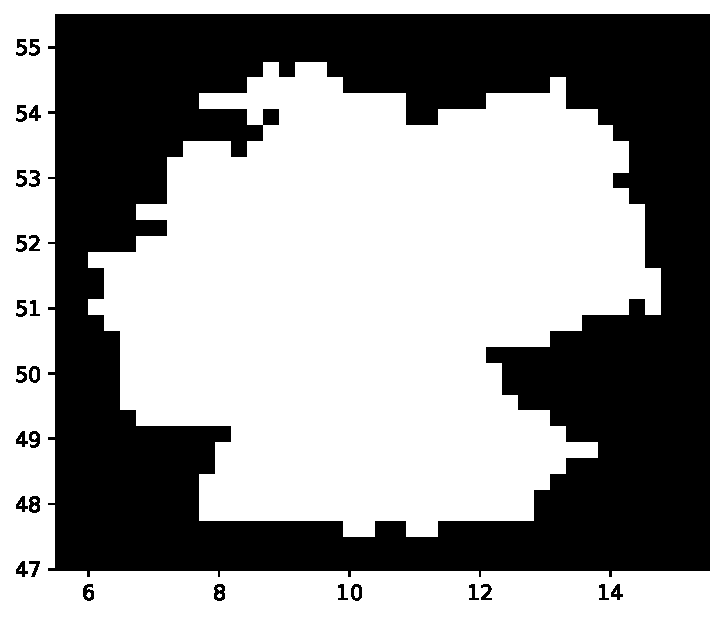
\includegraphics[width=.7\columnwidth]{plots/isin}%
\caption{This figure shows the 2D boolean numpy.ndarray used to filter grid squares that are within germany. It was created by using a shapefile of germany (TODO insert source \url{https://ec.europa.eu/eurostat/cache/GISCO/distribution/v2/nuts/nuts-2016-files.html}) and checking for each point of the grid if it is within the shapefile. (TODO shorter explanation, put explanation in text)}%
\label{fig:isin}%
\end{figure}

\begin{figure}[h!]%
\centering
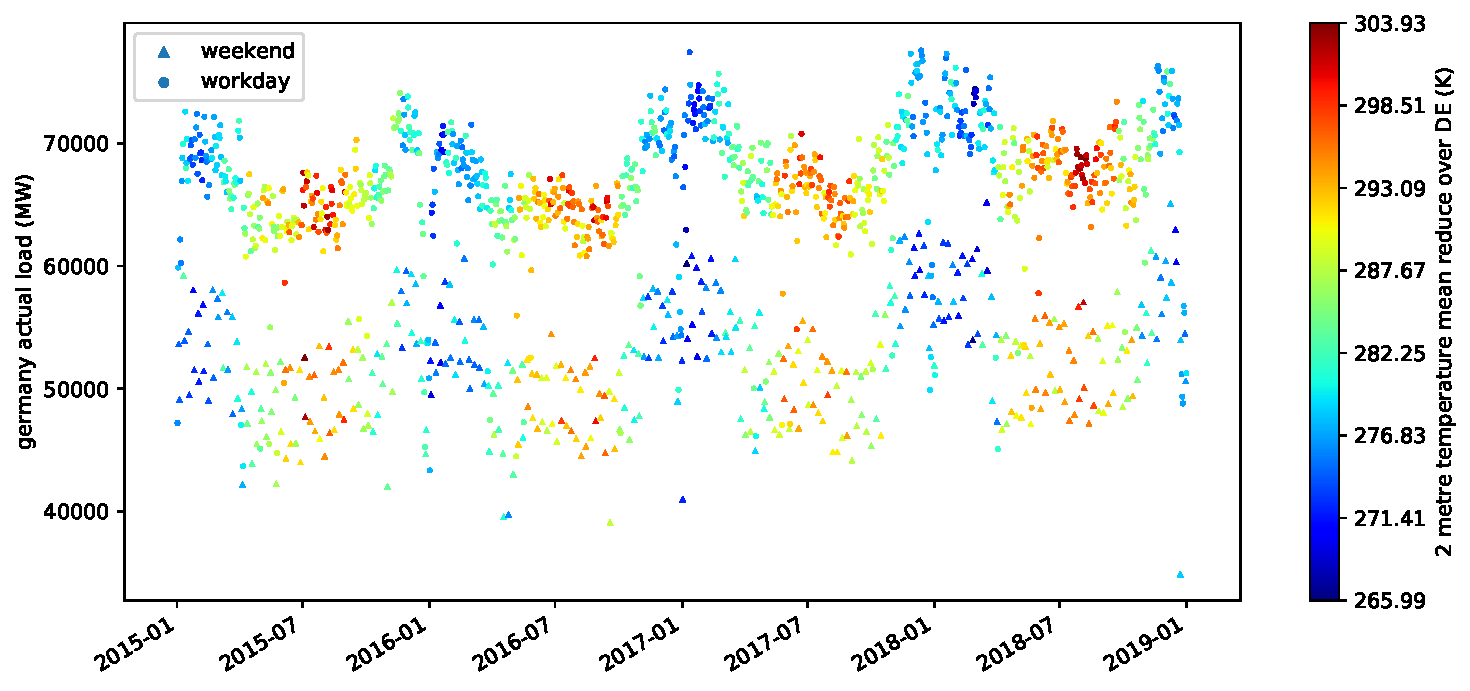
\includegraphics[width=.7\columnwidth]{plots/t2m_mean_2015010112_2018123112_24F}%
\caption{This figure shows a plot of the mean temperature in germany from 2015/1/1 to 2018/12/31 with one value per day at 12am utc time.}%
\label{fig:t2m_mean_2015010112_2018123112_24F}%
\end{figure}

\begin{table}[h!]%
\rowcolors{2}{gray!25}{white}
\centering
\footnotesize
\begin{tabular}{llrr}
\tablehead variable name & \tablehead units & \tablehead min & \tablehead max \\\hline
10 metre U wind component & m s**-1 & -18.56 & 21.92 \\
10 metre V wind component & m s**-1 & -21.51 & 20.00 \\
2 metre temperature & K & 240.97 & 313.26 \\
Leaf area index, high vegetation & m**2 m**-2 & 0.00 & 4.90 \\
Leaf area index, low vegetation & m**2 m**-2 & 0.00 & 3.84 \\
Low cloud cover & (0 - 1) & 0.00 & 1.00 \\
Soil temperature level 1 & K & 257.91 & 313.64 \\
Surface latent heat flux & J m**-2 & -2203977.00 & 359411.00 \\
Surface net thermal radiation & J m**-2 & -663417.00 & 142945.02 \\
Surface sensible heat flux & J m**-2 & -1703159.00 & 801354.00 \\
Total cloud cover & (0 - 1) & 0.00 & 1.00 \\
Total column rain water & kg m**-2 & 0.00 & 2.73 \\
Total sky direct solar radiation at surface & J m**-2 & -0.12 & 3088320.00 \\
\end{tabular}
\caption{List of exogenous weather variables used to forecast the load including min, max values.}
\label{tab:wvars}
\end{table}


\subsection{Load data}


%Describe the data set you are using. Use appropriate visualization (\eg graphs, statistical summaries \etc) to help the reader get to know your data set.

\Cref{tab:wvars} is an example table. Remember to use full sentences in your caption and explain everything one can see in the table there as well. You can of course also use a simpler format for your table.

%\begin{table}[h!]%
%\caption{Example table with rotated table heads to save space and two different row colours to ease the readability.}
%\rowcolors{2}{gray!25}{white}
%\centering
%\footnotesize
%\begin{tabular}{lll}
%\toprule \noalign{\smallskip}
%\rottblhead{\tablehead Header 1} & \rottblhead{\tablehead Header 2} & \rottblhead{\tablehead Header 3} \\ \midrule
%entry 1 & entry 2 & entry 3 \\ 
%entry 1 & entry 2 & entry 3 \\ 
%entry 1 & entry 2 & entry 3 \\ 	\bottomrule
%\end{tabular}
%\label{tab:example}
%\end{table}


\section{Programming part}

\subsection{Programming Language}

For the programming part, Python3.6+ has been chosen, as there is a variety of libraries to process all used file formats and because it tends to be a time saving language, also for visualization.\\

\subsection{Documentation}

In regard to coding styles, especially when it comes to docstrings, the numpy conventions were used. The three major points for this were first, that it is a popular and often used style, then it is also a visually oriented style which means, that it is easy to read and last it is supported by several (TODO check which, sphinx?!) autodoc tools that create a HTML based documentation from existing source code with docstrings.\\


\section{Results}

Describe the results you have obtained using your methods described above. Again use proper visualization methods.

\subsection{Experiment 1}

\dots

\subsection{Experiment 2}

\dots